\chapter{Introduction to Operating Systems}

\chapterquote{``An operating system is the most important software layer between hardware and applications.''}{Operating Systems Principle}

\section{Chapter Overview}

This chapter introduces the foundational concepts of Operating Systems (OS), one of the most important subjects in Software Development Engineer (SDE) interviews. Understanding operating systems helps engineers write efficient software, debug performance issues, reason about concurrency, and design scalable systems.

Major technology companies such as Amazon, Google, Microsoft, Meta, Uber, Netflix, Atlassian, Apple, and Bloomberg frequently ask operating system questions during interviews.

\section{Learning Objectives}

After completing this chapter, you should be able to:

\begin{itemize}
\item Explain what an Operating System is.
\item Describe major goals of operating systems.
\item Understand the evolution of operating systems.
\item Compare batch, multiprogramming, and time-sharing systems.
\item Understand distributed, real-time, and embedded operating systems.
\item Explain kernel responsibilities.
\item Differentiate user mode and kernel mode.
\item Understand system calls.
\item Explain the OS boot process.
\item Discuss why operating systems matter for software engineers.
\end{itemize}

%====================================================
\section{What is an Operating System?}
%====================================================

\subsection{Definition}

An \textbf{Operating System (OS)} is system software that manages computer hardware and software resources and provides services to applications.

It acts as an intermediary between:

\begin{itemize}
\item Users
\item Applications
\item Hardware
\end{itemize}

\begin{figure}[H]
\centering
\begin{tikzpicture}
\node[draw, rectangle, minimum width=5cm] (user) {Users};
\node[draw, rectangle, below=0.8cm of user, minimum width=5cm] (app) {Applications};
\node[draw, rectangle, below=0.8cm of app, minimum width=5cm] (os) {Operating System};
\node[draw, rectangle, below=0.8cm of os, minimum width=5cm] (hw) {Hardware};

\draw[->] (user) -- (app);
\draw[->] (app) -- (os);
\draw[->] (os) -- (hw);
\end{tikzpicture}
\caption{Operating System as an Interface}
\end{figure}

\subsection{Simple Analogy}

Consider a restaurant:

\begin{itemize}
\item Customers = Users
\item Waiter = Operating System
\item Kitchen = Hardware
\end{itemize}

Customers never directly communicate with the kitchen. The waiter coordinates requests and responses.

Similarly, applications do not directly access hardware. The operating system manages all interactions.

\subsection{Examples of Operating Systems}

\begin{itemize}
\item Linux
\item Windows
\item macOS
\item Android
\item iOS
\item FreeBSD
\item RTLinux
\item VxWorks
\end{itemize}

%====================================================
\section{Goals of an Operating System}
%====================================================

The primary goals of an operating system are:

\subsection{Convenience}

Provide an easy environment for running applications.

\subsection{Efficiency}

Utilize hardware resources efficiently.

\subsection{Resource Sharing}

Allow multiple users and programs to share resources safely.

\subsection{Reliability}

Prevent crashes and ensure system stability.

\subsection{Security}

Protect users and resources from unauthorized access.

\subsection{Scalability}

Support growth in users, processes, and hardware.

\begin{table}[H]
\centering
\begin{tabular}{|p{4cm}|p{8cm}|}
\hline
Goal & Description \\
\hline
Convenience & Simplifies application development \\
\hline
Efficiency & Maximizes CPU and memory usage \\
\hline
Reliability & Ensures correct operation \\
\hline
Security & Protects data and resources \\
\hline
Scalability & Handles increasing workloads \\
\hline
\end{tabular}
\caption{Goals of an Operating System}
\end{table}

%====================================================
\section{Evolution of Operating Systems}
%====================================================

Operating systems evolved through several stages.

\begin{enumerate}
\item No Operating System
\item Batch Systems
\item Multiprogramming Systems
\item Time-Sharing Systems
\item Personal Computer Operating Systems
\item Distributed Systems
\item Mobile Operating Systems
\item Cloud and Container-Oriented Systems
\end{enumerate}

\begin{figure}[H]
\centering
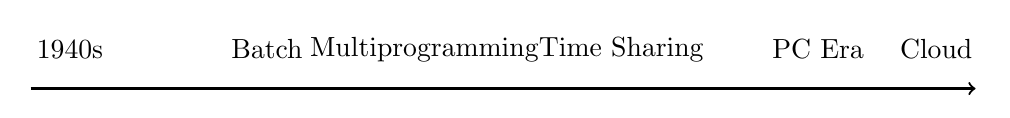
\begin{tikzpicture}
\draw[->, thick] (0,0) -- (12,0);

\node at (0.5,0.5) {1940s};
\node at (3,0.5) {Batch};
\node at (5,0.5) {Multiprogramming};
\node at (7.5,0.5) {Time Sharing};
\node at (10,0.5) {PC Era};
\node at (11.5,0.5) {Cloud};

\end{tikzpicture}
\caption{Evolution of Operating Systems}
\end{figure}

%====================================================
\section{Batch Systems}
%====================================================

\subsection{Definition}

Batch systems execute jobs in batches without user interaction.

\subsection{Working}

\begin{enumerate}
\item User submits jobs.
\item Jobs are grouped.
\item OS executes them sequentially.
\end{enumerate}

\subsection{Advantages}

\begin{itemize}
\item Simple implementation
\item Better CPU utilization than manual execution
\end{itemize}

\subsection{Disadvantages}

\begin{itemize}
\item No interaction
\item Long waiting time
\end{itemize}

\subsection{Example}

Early IBM mainframe systems.

%====================================================
\section{Multiprogramming Systems}
%====================================================

\subsection{Definition}

Multiple programs reside in memory simultaneously.

When one process waits for I/O, another process uses the CPU.

\subsection{Goal}

Increase CPU utilization.

\begin{figure}[H]
\centering
\begin{tikzpicture}
\node[draw] (cpu) {CPU};

\node[draw,left=3cm of cpu] (p1) {P1};
\node[draw,above=1cm of p1] (p2) {P2};
\node[draw,below=1cm of p1] (p3) {P3};

\draw[->] (p1) -- (cpu);
\draw[->] (p2) -- (cpu);
\draw[->] (p3) -- (cpu);
\end{tikzpicture}
\caption{Multiprogramming Concept}
\end{figure}

\subsection{Example}

Early UNIX systems.

%====================================================
\section{Time Sharing Systems}
%====================================================

\subsection{Definition}

Time-sharing systems allow multiple users to interact with a computer simultaneously.

\subsection{How It Works}

CPU time is divided into small slices called \textbf{time quanta}.

\subsection{Advantages}

\begin{itemize}
\item Interactive computing
\item Improved user experience
\item Fair CPU allocation
\end{itemize}

\subsection{Examples}

\begin{itemize}
\item UNIX
\item Linux
\item Windows
\end{itemize}

%====================================================
\section{Distributed Operating Systems}
%====================================================

\subsection{Definition}

A distributed OS manages multiple computers and presents them as a single system.

\subsection{Goals}

\begin{itemize}
\item Resource sharing
\item Fault tolerance
\item Scalability
\end{itemize}

\subsection{Examples}

\begin{itemize}
\item Amoeba
\item Plan 9
\item Modern cloud infrastructures
\end{itemize}

%====================================================
\section{Real-Time Operating Systems}
%====================================================

\subsection{Definition}

A Real-Time Operating System (RTOS) guarantees response within strict timing constraints.

\subsection{Types}

\begin{enumerate}
\item Hard Real-Time
\item Soft Real-Time
\end{enumerate}

\begin{table}[H]
\centering
\begin{tabular}{|p{5cm}|p{5cm}|}
\hline
Hard RTOS & Soft RTOS \\
\hline
Missing deadline unacceptable & Missing deadline tolerated \\
\hline
Aircraft systems & Video streaming \\
\hline
\end{tabular}
\caption{Hard vs Soft RTOS}
\end{table}

\subsection{Examples}

\begin{itemize}
\item VxWorks
\item QNX
\item RTLinux
\end{itemize}

%====================================================
\section{Embedded Operating Systems}
%====================================================

\subsection{Definition}

Embedded operating systems run on dedicated devices.

\subsection{Characteristics}

\begin{itemize}
\item Low memory footprint
\item High reliability
\item Energy efficient
\end{itemize}

\subsection{Examples}

\begin{itemize}
\item FreeRTOS
\item Embedded Linux
\item Zephyr
\end{itemize}

%====================================================
\section{Components of an Operating System}
%====================================================

Major OS components include:

\begin{itemize}
\item Process Management
\item Memory Management
\item File System
\item I/O Management
\item Security
\item Networking
\item Device Drivers
\end{itemize}

\begin{figure}[H]
\centering
\begin{tikzpicture}

\node[draw,rectangle] (os) {Operating System};

\node[draw,below left=1.5cm and 2cm of os] (proc) {Process Mgmt};
\node[draw,below=1.5cm of os] (mem) {Memory Mgmt};
\node[draw,below right=1.5cm and 2cm of os] (fs) {File System};

\draw (os)--(proc);
\draw (os)--(mem);
\draw (os)--(fs);

\end{tikzpicture}
\caption{Major OS Components}
\end{figure}

%====================================================
\section{Kernel Overview}
%====================================================

\subsection{Definition}

The kernel is the core component of an operating system.

It manages:

\begin{itemize}
\item CPU
\item Memory
\item Devices
\item Processes
\end{itemize}

\subsection{Kernel Responsibilities}

\begin{itemize}
\item Process scheduling
\item Memory management
\item Interrupt handling
\item Device communication
\item Security enforcement
\end{itemize}

\subsection{Types of Kernels}

\begin{table}[H]
\centering
\begin{tabular}{|p{3cm}|p{8cm}|}
\hline
Monolithic & Services inside kernel space \\
\hline
Microkernel & Minimal kernel functionality \\
\hline
Hybrid & Combination approach \\
\hline
\end{tabular}
\caption{Kernel Types}
\end{table}

\subsection{Examples}

Linux uses a monolithic kernel.

Windows uses a hybrid kernel.

%====================================================
\section{User Mode vs Kernel Mode}
%====================================================

\begin{table}[H]
\centering
\begin{tabular}{|p{4cm}|p{5cm}|p{5cm}|}
\hline
Feature & User Mode & Kernel Mode \\
\hline
Privilege & Restricted & Full Access \\
\hline
Hardware Access & No & Yes \\
\hline
Crash Impact & Process Only & Entire System \\
\hline
\end{tabular}
\caption{User Mode vs Kernel Mode}
\end{table}

\begin{figure}[H]
\centering
\begin{tikzpicture}

\node[draw,rectangle,minimum width=5cm] (u) {User Space};
\node[draw,rectangle,below=1cm of u,minimum width=5cm] (k) {Kernel Space};

\draw[->] (u)--(k);

\end{tikzpicture}
\caption{Mode Transition}
\end{figure}

%====================================================
\section{System Calls}
%====================================================

System calls provide an interface between applications and the operating system.

\subsection{Examples}

Linux:

\begin{verbatim}
read()
write()
fork()
exec()
open()
close()
\end{verbatim}

Windows:

\begin{verbatim}
CreateProcess()
ReadFile()
WriteFile()
\end{verbatim}

\subsection{Flow}

Application $\rightarrow$ System Call $\rightarrow$ Kernel

%====================================================
\section{Boot Process Overview}
%====================================================

\begin{enumerate}
\item Power On
\item BIOS/UEFI Initialization
\item Bootloader Execution
\item Kernel Loading
\item Hardware Initialization
\item System Services Start
\item User Login
\end{enumerate}

\begin{figure}[H]
\centering
\begin{tikzpicture}

\node[draw] (p) {Power On};
\node[draw,right=2cm of p] (b) {BIOS/UEFI};
\node[draw,right=2cm of b] (bl) {Bootloader};
\node[draw,right=2cm of bl] (k) {Kernel};

\draw[->] (p)--(b);
\draw[->] (b)--(bl);
\draw[->] (bl)--(k);

\end{tikzpicture}
\caption{Boot Sequence}
\end{figure}

%====================================================
\section{Operating System Services}
%====================================================

Operating systems provide:

\begin{itemize}
\item Program execution
\item I/O operations
\item File manipulation
\item Communication
\item Error detection
\item Resource allocation
\item Security
\end{itemize}

%====================================================
\section{Why Operating Systems Matter for SDEs}
%====================================================

\subsection{Interview Perspective}

Companies ask OS questions because engineers must understand:

\begin{itemize}
\item Concurrency
\item Threading
\item Memory usage
\item Scheduling
\item Performance bottlenecks
\item Scalability
\end{itemize}

\subsection{Real-World Examples}

\begin{itemize}
\item High CPU usage debugging
\item Memory leaks
\item Deadlock investigation
\item Container scheduling
\item Distributed systems design
\end{itemize}

\subsection{Interview Tip}

Always connect operating system concepts with:

\begin{itemize}
\item Performance
\item Scalability
\item Reliability
\item Security
\end{itemize}

%====================================================
\section{Key Takeaways}
%====================================================

\begin{itemize}
\item Operating systems manage hardware resources.
\item Kernels are the core of operating systems.
\item System calls enable user-kernel interaction.
\item Multiprogramming improves CPU utilization.
\item Time sharing enables interactivity.
\item RTOS systems focus on deadlines.
\item Distributed systems provide scalability.
\item OS knowledge is critical for SDE interviews.
\end{itemize}

%====================================================
\section{15 Interview Questions with Answers}
%====================================================

\begin{enumerate}
\item What is an operating system?\\
Answer: System software managing hardware and providing services.

\item What are the main goals of an OS?\\
Answer: Convenience, efficiency, security, reliability.

\item What is a kernel?\\
Answer: Core component managing resources.

\item What is multiprogramming?\\
Answer: Multiple programs in memory simultaneously.

\item What is time sharing?\\
Answer: CPU sharing through time slices.

\item Difference between user and kernel mode?\\
Answer: Privilege level and hardware access.

\item What is a system call?\\
Answer: Interface to request kernel services.

\item What is a distributed OS?\\
Answer: OS managing multiple machines as one.

\item What is RTOS?\\
Answer: OS with deterministic response times.

\item What is a bootloader?\\
Answer: Program loading the kernel.

\item Why are interrupts important?\\
Answer: Enable event-driven processing.

\item Linux kernel type?\\
Answer: Monolithic.

\item Windows kernel type?\\
Answer: Hybrid.

\item Why does OS scheduling matter?\\
Answer: Efficient CPU allocation.

\item Why do SDE interviews ask OS questions?\\
Answer: To evaluate systems understanding.
\end{enumerate}

%====================================================
\section{15 MCQs with Answers}
%====================================================

\begin{enumerate}
\item OS primarily acts as:
\begin{enumerate}
\item Compiler
\item Interface between hardware and applications
\item Database
\item Browser
\end{enumerate}
Answer: B

\item Kernel runs in:
A) User mode
B) Kernel mode
Answer: B

\item Linux kernel is:
A) Microkernel
B) Hybrid
C) Monolithic
D) Exokernel
Answer: C

\item Multiprogramming improves:
Answer: CPU Utilization

\item RTOS stands for:
Answer: Real-Time Operating System

\item System calls are used for:
Answer: Accessing OS services

\item Time-sharing systems use:
Answer: Time quanta

\item BIOS executes before:
Answer: Kernel

\item Embedded OS targets:
Answer: Dedicated devices

\item User mode has:
Answer: Restricted privileges

\item Kernel mode has:
Answer: Full privileges

\item Process management is handled by:
Answer: OS

\item Example RTOS:
Answer: VxWorks

\item Example desktop OS:
Answer: Windows

\item Example distributed OS:
Answer: Amoeba
\end{enumerate}

%====================================================
\section{Revision Notes}
%====================================================

\begin{itemize}
\item OS = Resource Manager + Abstraction Layer.
\item Kernel is the heart of the OS.
\item User mode is restricted.
\item Kernel mode has full access.
\item System calls cross privilege boundaries.
\item Multiprogramming increases CPU utilization.
\item Time sharing improves responsiveness.
\item RTOS guarantees timing constraints.
\item Embedded OS focuses on resource efficiency.
\item Distributed OS improves scalability.
\end{itemize}

%====================================================
\section{Cheat Sheet}
%====================================================

\begin{center}
\begin{tabular}{|p{5cm}|p{8cm}|}
\hline
Operating System & Resource manager and abstraction layer \\
\hline
Kernel & Core OS component \\
\hline
System Call & Interface to kernel services \\
\hline
Multiprogramming & Multiple programs in memory \\
\hline
Time Sharing & CPU divided into quanta \\
\hline
RTOS & Deadline-oriented OS \\
\hline
Distributed OS & Multiple machines appear as one \\
\hline
User Mode & Restricted execution \\
\hline
Kernel Mode & Privileged execution \\
\hline
Boot Process & BIOS $\rightarrow$ Bootloader $\rightarrow$ Kernel \\
\hline
\end{tabular}
\end{center}